\documentclass{standalone}
\usepackage{tikz}
\usetikzlibrary{calc,patterns,decorations.pathmorphing,decorations.markings}

% node, begin anchor, end anchor, name
\newcommand{\makepoints}[3]{
    \foreach \k in {1, ..., \points}
    {
        \pgfmathsetmacro{\dist}{\k * (1 / (\points + 1))}
        \coordinate (#1 \k) at ($(#2)!\dist!(#3)$);
    }
}

\begin{document}

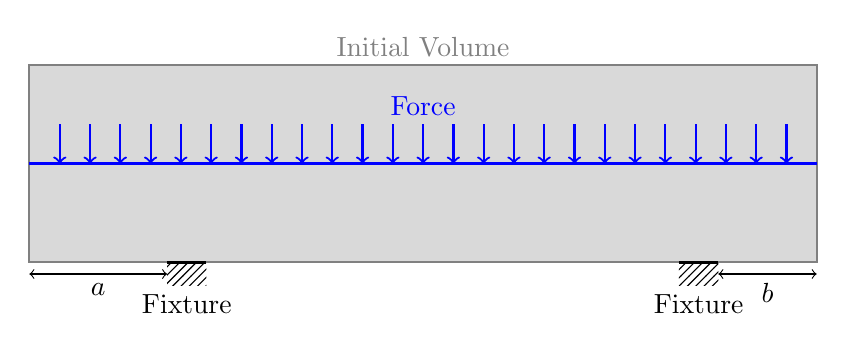
\begin{tikzpicture}[every node/.style={draw,outer sep=0pt,thick}]

% number of arrows between nodes
\pgfmathtruncatemacro{\points}{25}
        
\tikzstyle{ground}=[fill,pattern=north east lines,draw=none,minimum width=1cm,minimum height=0.3cm]


\node (M) [gray,label={[gray]Initial Volume},minimum width=10cm,minimum height=2.5cm,fill=gray!30] {};
\node (floor1) at (M.south east)[ground,label={below:Fixture},minimum width=.5cm,yshift=-0.15cm,xshift=-1.5cm] {};
\draw[very thick] (floor1.north east) -- (floor1.north west);
\node (floor2) at (M.south west)[ground,label={below:Fixture},minimum width=.5cm,yshift=-0.15cm,xshift=2cm] {};
\draw[very thick] (floor2.north east) -- (floor2.north west);

\draw[<->] 	let	\p1 = (M.west), 
			\p2 = (floor2.west) 
		in  (\x1,\y2) -- node[draw=none,below]{$a$} (\x2,\y2);
		
\draw[<->] 	let	\p1 = (M.east), 
			\p2 = (floor1.east) 
		in  (\x1,\y2) -- node[draw=none,below]{$b$} (\x2,\y2);		

\coordinate (attackareaStart) at (M.east);
\coordinate (attackareaEnd) at (M.west);
\coordinate (forceStart) at ($(attackareaStart)+(0,.5)$);
\coordinate (forceEnd) at ($(attackareaEnd)+(0,.5)$);
\makepoints{bottom}{attackareaStart}{attackareaEnd}
\makepoints{top}{forceStart}{forceEnd}
% arrows
\foreach \i in {1, ..., \points} {
    \draw [->,blue,thick] (top \i) -- (bottom \i);
}
\draw[very thick,blue](attackareaStart)--(attackareaEnd);
\node[blue,above,draw=none](force) at ($.5*(forceStart)+.5*(forceEnd)$){Force};
\end{tikzpicture}

\end{document}